%FOR PDFLATEX USE ONLY
\documentclass[a4paper,12pt]{article}

\usepackage{amssymb,amsmath} %math symbols

\usepackage[margin=2cm]{geometry} %paper geometry

\usepackage[utf8]{inputenc} %allows unicode (including russian) source file
\usepackage[russian]{babel} %docment in russian-style
\usepackage[utf8]{inputenc}
%\usepackage[unicode]{hyperref} %links inside of the text
\usepackage[pdftex]{graphicx} %includegraphics pictures
\usepackage{cmlgc} %bold text

\usepackage{array} %arrays

%\usepackage{wrapfig}
%\usepackage{array}
%\usepackage{lipsum}
%\usepackage{esvect}
%\usepackage{hyperref}

\usepackage{subfig}
%\usepackage{calc}
%\usepackage{pgfplots,tikz,circuitikz}
%\usepackage{tkz-euclide}

\begin{document}

\begin{center}
  \LARGE{Работа 4.7.2}\\[0.2cm]
  \LARGE{Эффект Поккельса}\\[0.2cm]
  \large{Стрижак Даниил}\\[0.2cm]
\end{center}  
  

\section{Аннотация}

В работе предстоит исследовать интерференцию рассеянного света, прошедшего кристалл; наблюдать изменение характера поляризации света при наложении на кристалл электрического поля.

\section{Теоретические сведения}

Эффект Поккельса -- изменение показателя преломления света в кристалле под действием электрического поля.\\
Рассмотрим кристалл ниобата лития $\text{LiNbO}_3$ с цетрольноосевой симметрией вдоль оси $Z$. Для световой волны с $\mathbf{E}$ перпендикулярно $Z$ показатель преломления будет $n_o$, а для волны с $\mathbf{E}$ вдоль $Z$ -- $n_e$. В случае, когда луч света идёт под углом $\theta$ к оси, есть два значение показателя преломления $n_1$ и $n_2$: $n_1 = n_o$ для волны с $\mathbf{E}$ перпендикулярным плоскости $(\mathbf{k},\mathbf{Z})$ (обыкновенная волна) и $n_2$ для волны с $\mathbf{E}$ в этой плоскости (необыкновенная волна). В последнем случае
\begin{equation}
\dfrac{1}{n_2^2}=\dfrac{\cos^2 \theta}{n_0^2}+\dfrac{\sin^2 \theta}{n_e^2}.
\end{equation}


\begin{minipage}{0.47\textwidth}
Если перед кристаллом, помещённым между поляроидами, расположить линзу или матовую пластинку, то на экране за поляроидом мы увидим тёмные концентрические окружности -- рещультат интерфернции обыкновенной и необыкновенной волн. При повороте выходного поляроида на $90^\circ$ картина меняется с позитива на негатив (на месте светлых пятен тёмные и наоборот). В случаи, когда разрешённое направление анализатора перпендикулярно поляризации лазерного излучения, радиус тёмного кольца с номером $m$ равен
\end{minipage}
\begin{minipage}{0.05\textwidth}
\
\end{minipage}
\begin{minipage}{0.47\textwidth}
\begin{center}
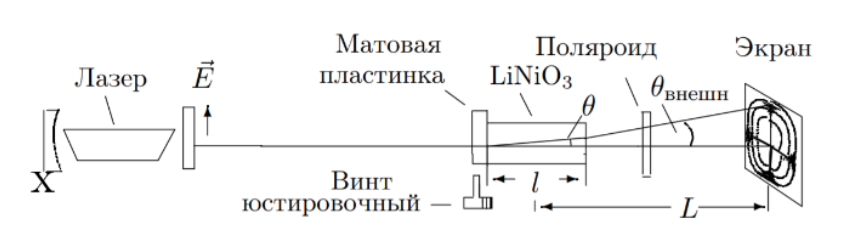
\includegraphics[width = \textwidth]{1.png}
\end{center}
\vspace{-40ptx}
\begin{center}
Схема для наблюдения интерфереционной картины.
\end{center}
\end{minipage}
\begin{equation}
r_m^2 = \dfrac{\lambda}{l} \dfrac{(n_oL)^2}{n_0 - n_e}m,
\end{equation}
где $L$ -- расстояние от центра кристалла до экрана, $l$ -- длина кристалла.\\
Теперь поместим кристалл в постоянное электрическое поле $E_{\text{эл}}$, направленное вдоль оси $X$, перпендикулярной $Z$. Показатель преломления для луча, распространяющего вдоль $Z$, всегда $n_o$. В плоскости $(X,Y)$ возникают два главных направления под углами $45^\circ$ к $X$ и $Y$ с показателями преломления $n_0 - \Delta n$ и $n_o + \Delta n$ (быстрая и медленная ось), причём $\Delta n = A E_{\text{эл}}$. Для поляризованного вертикально света и анализатора, пропускающего горизонтальную поляризацию, на выходе интенсивность на выходе будет иметь вид
\begin{equation}
I_{\text{вых}} = I_0 \sin^2 \left(\dfrac{\pi}{2} \dfrac{U}{U_{\lambda/2}} \right),
\end{equation}
где $U_{\lambda/2} = \frac{\lambda}{4A}\frac{d}{l}$ -- \textit{полуволновое напряжение}, $d$ -- поперечный размер кристалла.  При напряжении $U = E_{\text{эл}}d$ равном полуволновому сдвиг фаз между двумя волнами равен $\pi$, а интенсивность света на выходе максимальна. 


\begin{wrapfigure}{r}{0.45\textwidth}
\begin{center}
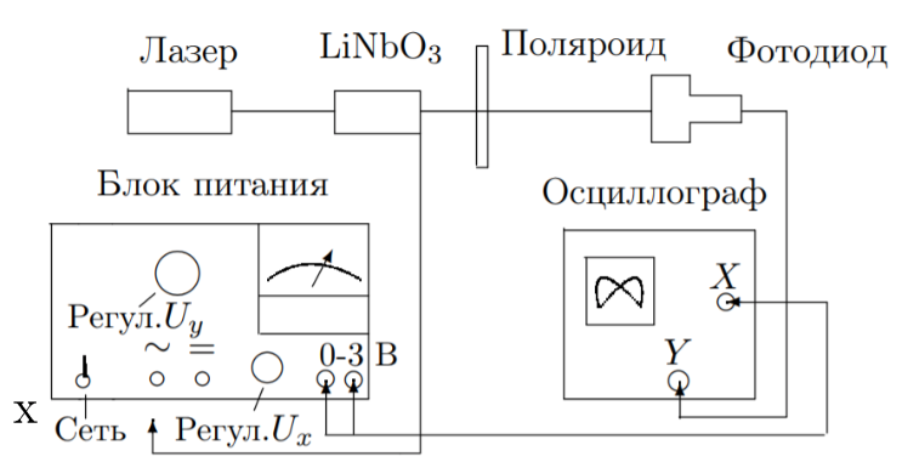
\includegraphics[width = 0.45\textwidth]{2.png}
\end{center}
\vspace{-40ptx}
\caption*{Схема установки.}
\end{wrapfigure}
На Рис. 2 представлена схема всей установки (оптическая часть изорбажена на Рис. 1). Свет лазера, проходя через сквозь пластину, рассеивается и падает на двоякопреломляющий кристалл. На экране за поляроидом видна интерференционная картина. Убрав рассеивающую пластину и подавая на кристалл постоянное напряжение, можно величиной напряжения влиять на поляризацию луча, вышедшего из кристалла. Заменив экран фотодиодом и подав на кристалл переменное напряжение, можно исследовать поляризацию с помощью осциллографа.


\section{Результаты измерений и обработка данных}

Соберем схему и подготовим приборы к работе, следуя техническому описанию, расположенному на установке.

	
	Схема наблюдения интерференционной картины приведена на рисунке \ref{shema}. Свет лазера, поляризованный в вертикальной плоскости, рассеивается на матовой пластинке и проходит через двоякопреломляющий кристалл. На выходе из кристалла стоит поляроид. Параметры установки: размеры кристалла $3 \times 3 \times 26$ мм, длина волны гелий-неонового лазера $\lambda = 0,63$ мкм, показатель преломления $n_o = 2,29$, расстояние до экрана от центра кристалла $L = (76 \pm 1)$ см, $l = 26$ мм - длина кристалла вдоль оптической оси.
	
Соберем установку по схеме на рисунке 1, предварительно убедившись в вертикальной поляризации лазера. Лазер установим так, чтобы в отсутствии кристалла излучение через него не проходило. Оптимальное расстояние $L$ от экрана до центра кристалла определим экспериментально, центр интерференционной картины совместим с изображением луча в отсутствие матовой пластинки. При повороте анализатора на $90^\circ$ градусов от исходного положения картинка на экране меняется на негативную, что соответствует смене разрешенной выходной поляризации и, следовательно, условиям на темные кольца. 
	
	Снимем зависимость радиусов темных концентрических колец от номера максимума $r_m(m)$. Для большей точности измерений отметим положения колец на экране вдоль прямой карандашом. Погрешность величины $r_m$ примем равной $0,2$ см из-за расплывчатости картинки. Результаты измерений занесены в таблицу 1. 
	
\newpage
	
	
	
	На основе таблицы 1 построен график зависимости квадрата радиуса кольца от номера соответствующего минимума $r_m^2(m)$, изображенный на рисунке 1. Погрешность $r_m^2$ рассчитана по формуле произведения погрешностей. 

\begin{minipage}{0.47\textwidth}	
	\begin{center}
\begin{tabular}{|c|c|c|c|}
\hline
$m$ &$r_m$, см &  $r_m^2$, см^2 &$\Delta r_m^2$, см^2\\
\hline
1 &2.7&7.3& 0.8\\
\hline
2&3.7&13.7&1.0\\
\hline
3&4.9&24.0&1.4\\
\hline
4&5.6&31.4&1.6\\
\hline
5&6.3&39.7&1.8\\
\hline
6&7.1&50& 2\\
\hline
7&7.5&56&2\\
\hline
\end{tabular}
\end{center}	
\end{minipage}	
\begin{minipage}{0.47\textwidth}
\begin{center}
		\begin{tikzpicture}[scale = 1.0]
		\begin{axis}[
		axis lines = left,
		ylabel = {P},
		xlabel = {$\rho$},
		minor grid style={black, line width=0.05pt},
		major grid style={solid,black, line width=0.3pt},
		xmin=0, xmax=8,
		ymin=3, ymax=60,
		ymajorgrids = true,
		xmajorgrids = true,
		yminorgrids = true,
		xminorgrids = true,
		minor tick num = 4
		]
		\addplot+[only marks ] plot[error bars/.cd, y dir=both, y explicit]
		coordinates {
			(1,7.3)
			(2,13.7)
			(3,24)
			(4,31.4)
			(5,39.7)
			(6,50)
			(7,56)
		};
		
		\addplot[blue, domain=0:8]{8.43*x - 3};
		\end{axis}

		\end{tikzpicture}
		
\end{center}
\end{minipage}
	
	Экспериментальные точки хорошо на прямую $r_m^2 = bm + a$, что соответствует теоретической зависимости (2). Проведем ее методом наименьших квадратов, воспользовавшись привычными формулами для коэффициентов прямой и их погрешностей.
	
	Для коэффициента наклона имеем: 
	
	\[ b = \frac{\lambda}{l} \frac{(n_oL)^2}{(n_o - n_e)} = (8,43 \pm 0,19) \text{ см}^2 \] 
	
	Выразим двулучепреломление ниобата лития $n_o - n_e$:
	
	\[ n_o - n_e = \frac{\lambda}{l}\frac{(n_oL)^2}{b} = (87 \pm 3) \cdot 10^{-3} \]
	
	Для вычисления использовались параметры установки, описанные в начале раздела. Считаем, что вклад в погрешность дают непосредственно измеренные величины: длина от центра кристалла до экрана $L$ и коэффициент $b$.
	
	\subsection*{Изменение характера поляризации света \\ при наличии внешнего поля}
	
	
	
	Соберем схему как на рисунке 2 и подключим разъем блока питания на постоянное напряжение. Увеличивая напряжение с нулевого значения, проследим за изменением яркости пятна на экране. 
	
	Для скрещенных поляризаций при напряжениях $U = (2k - 1)U_{\lambda/2}$ наблюдается максимум интенсивности, при $U = 2kU_{\lambda/2}$ - минимум, здесь $k$ - натуральное число. Для параллельных поляризаций ситуация противоположная. 
	
	Напряжения, соответствующие последовательным экстремумам интенсивности для разных поляризаций, содержатся в таблице \ref{vol}.	В 100 делениях шкалы блока питания 1,5 кВ. Погрешность измерения напряжения примем равной 1 делению, или 15 В. 
	
\newpage
	
	\begin{center}
\begin{tabular}{|c|c|c|}
\hline
 &Скрещенные поляризации& Параллельные поляризации\\
\hline
$U_{\lambda/2}$, дел &30&28\\
\hline
$U_{\lambda/2}$, В&450&420\\
\hline
$U_{\lambda}$, дел&60&60\\
\hline
$U_{\lambda/2}$, В&900&900\\
\hline
$U_{3\lambda/2}$, дел&92&92\\
\hline
$U_{3\lambda/2}$, В&1380&1380\\
\hline
\end{tabular}
\end{center}

	По таблице \ref{vol} найдем среднее значение полуволнового напряжения; погрешность его определения складывается из приборной погрешности и случайной, сопоставимых по величине, поэтому оценим ее как $2\cdot 10$ В. 
	
	\[ U_{\lambda/2} = (46 \pm 2) \cdot 10 \text{ В} \] 
	
	При напряжении $U_{\lambda/4}$ интенсивности при скрещенной и параллельной поляризациях совпадают. Выставим экспериментальное значение напряжения $U_{\lambda/4} = U_{\lambda/2}/2 \approx 230$ В. При вращении анализатора интенсивность наблюдаемого пятна практически не меняется, что свидетельствует о круговой поляризации и подтверждает правильность расчетов.  
	
	Заменим в схеме, изображенной на рисунке \ref{full}, экран фотодиодом, подключим его к $Y$-входу осциллографа. На $X$-вход подадим переменное напряжение с блока питания. В режиме DUAL на экране осциллографа получаются фигуры Лиссажу, отвечающие зависимости $I(U)$. Она задается формулой (3) для скрещенных поляризаций и имеет вид синусоиды, взятой на симметричном отрезке, или формулой (4) для параллельных поляризаций и представляет собой косинусоиду. Таким образом, фигуры Лиссажу для разных поляризаций при одинаковом значении амплитуды напряжения $U$ отличаются по фазе на $\pi/2$.
	
	Определим полуволновое напряжение, измерив разность показаний между последовательными фигурами Лиссажу на экране, соответствующие экстремумам сигнала: 
	
	\[ U_{\lambda/2} \approx 30 \text{ дел} = 450 \text{ В} \]
	
	Фотографии наблюдаемых фигур Лиссажу для напряжений, кратным полуволновому, при параллельных поляризациях представлены на рисунке \ref{lis}.
	
	\begin{figure}[h]
		\begin{minipage}[h]{0.3\linewidth}
			\center{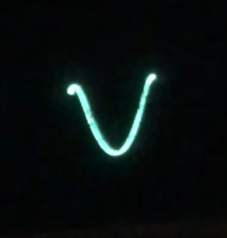
\includegraphics[width=0.9\linewidth]{photo1.png} \\ a)}
		\end{minipage}
		\hfill
		\begin{minipage}[h]{0.3\linewidth}
			\center{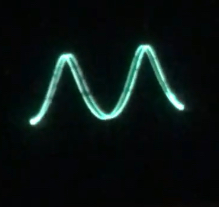
\includegraphics[width=0.9\linewidth]{photo2.png} \\ b)}
		\end{minipage}
		\hfill
		\begin{minipage}[h]{0.3\linewidth}
			\center{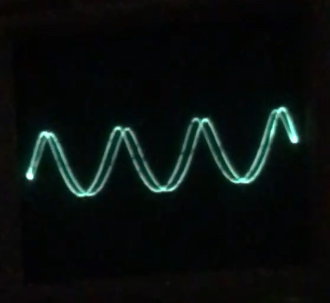
\includegraphics[width=0.9\linewidth]{photo3.png} \\ c)}
		\end{minipage}
		\caption{Фигуры Лиссажу для параллельных поляризаций при различных амплитудах напряжения $U$: (a) $U = U_{\lambda/2}$, (b) $U = U_{\lambda}$, (c) $U = U_{3\lambda/2}$ }
		\label{lis}
	\end{figure}

	
	\newpage
	\section{Вывод}
	
	В работе изучена интерференция рассеянного света, прошедшего кристалл ниобата лития: получена зависимость квадрата радиуса темного кольца интерференционной картины от номера минимума $r_m^2(m)$, с хорошей точностью являющаяся линейной (ошибка углового коэффициента 2\%), что согласуется с теорией при малых углах отклонения луча от оптической оси кристалла и близких значениях показателей преломления для обыкновенной и необыкновенной волн. Действительно, двулучепреломление кристалла $n_o - n_e$ составляет $(87 \pm 3)\cdot10^{-3}$, это значение соответствует литиевым кристаллам. 
	
	Рассмотрен эффект Поккельса: несколькими способами определено полуволновое напряжение, оно совпадает в пределах погрешности и равно $U_{\lambda/2} \approx 460$ В. Получены фигуры Лиссажу, отражающие зависимость интенсивности выходного сигнала от подаваемой амплитуды напряжения $I(U)$ при скрещенных и параллельных поляризациях. Картинки для поляризаций отличаются по фазе на $\pi/2$.
	
	\


\end{document}
